%%%%%%%%%%%%%%%%%%%%%%%%%%%%%%%%%%%%%%%%%%%%%%%%%%%%%%%%%%%%%%%%%%%%%%%%
%     LaTeX source code to approximate a NIST Technical report
%	  Instructions for authors: tinyurl.com/techpubsnist
%	DOI watermark will be added on final PDF
% 	Developed by K. Miller, kmm5@nist.gov
%	Last updated: 10-Oct-2017
%%%%%%%%%%%%%%%%%%%%%%%%%%%%%%%%%%%%%%%%%%%%%%%%%%%%%%%%%%%%%%%%%%%
\documentclass[12pt]{article}
\usepackage{adjustbox}
\usepackage{amsmath}
\usepackage{amsfonts}   % if you want the fonts
\usepackage{amssymb}    % if you want extra symbols
\usepackage{bm}
\usepackage{float}
\usepackage[hang,flushmargin,bottom]{footmisc} % footnote format
\usepackage{graphicx}   % need for figures		
\usepackage{mathptmx}
\usepackage{multicol}
\usepackage{physics}
\usepackage{rotating}
\usepackage{secdot}
\usepackage{siunitx} % Formats the units and values
\usepackage{tabulary}
%\usepackage{tablefootnote}
\usepackage{textgreek}
\usepackage{textcomp}
\usepackage{tikz}
\usepackage{titlesec}
\usepackage[utf8]{inputenc}
\usepackage{xcolor}
\titleformat{\section}{\normalsize\bfseries}{\thesection.}{1em}{}	% required for heading numbering style
\titleformat*{\subsection}{\normalsize\bfseries}

\usepackage{tocloft}	% change typeset, titles, and format list of appendices/figures/tables
\renewcommand{\cftdot}{}	
\renewcommand{\contentsname}{Table of Contents}
\renewcommand{\cftpartleader}{\cftdotfill{\cftdotsep}} % for parts
\renewcommand{\cftsecleader}{\cftdotfill{\cftdotsep}}
\renewcommand\cftbeforesecskip{\setlength{4pt}{}}
\addtolength{\cftfignumwidth}{1em}
\renewcommand{\cftfigpresnum}{\figurename\ }
\addtolength{\cfttabnumwidth}{1em}
\renewcommand{\cfttabpresnum}{\tablename\ }
\setlength{\cfttabindent}{0in}    %% adjust as you like
\setlength{\cftfigindent}{0in}

\usepackage{enumitem}         % to control spacing between bullets/numbered lists

\usepackage[numbers,sort&compress]{natbib} % format bibliography
\renewcommand{\bibsection}{}
\setlength{\bibsep}{0.0pt}

\usepackage[hidelinks]{hyperref} % hyperref package & removing outline from links

\usepackage{epstopdf} % converting EPS figure files to PDF

\usepackage{fancyhdr, lastpage}	% formatting document, calculating number of pages, formatting headers
\setlength{\topmargin}{-0.5in}
\setlength{\headheight}{39pt}
\setlength{\oddsidemargin}{0.25in}
\setlength{\evensidemargin}{0.25in}
\setlength{\textwidth}{6.0in}
\setlength{\textheight}{8.5in}

\usepackage{caption} % required for Figure labels
\captionsetup{font=small,labelfont=bf,figurename=Fig.,labelsep=period,justification=raggedright}

\newcommand*\textfrac[2]{
  \frac{{#1}}{{#2}}
}

\makeatletter
\def\@seccntformat#1{\@ifundefined{#1@cntformat}%
   {\csname the#1\endcsname\quad}%      default
   {\csname #1@cntformat\endcsname}%    enable individual control
}
\makeatother

%%%%%%%%%%% !!!!!! REQUIRED - FILL OUT METADATA HERE !!!!!!!! %%%%%%%%%%%%%%
%  	Report Number - fill in Report Number sent to you (see info below)
%   DOI Statement - fill in DOI sent to you
%   Month Year - fill in Month and Year of Publication
%%%%%%%%%%%%%%%%%%%%%%%%%%%%%%%%%%%%%%%%%%%%%%%%%%%%%%%%%%%%%%%%%%%%%%%%%%%%%%%%%%%%%%
\newcommand{\pubnumber}{XXXX}
\newcommand{\DOI}{https://doi.org/10.6028/NIST.TN.XXXX}
\newcommand{\monthyear}{October 2018}
%%%%%%%%%%%%%%%%%%%%%%%%%%%%%%%%%%%%%%%%%%%%%%%%%%%%%%%%%%%%%%%%%%%%
%   	BEGIN DOCUMENT
%%%%%%%%%%%%%%%%%%%%%%%%%%%%%%%%%%%%%%%%%%%%%%%%%%%%%%%%%%%%%%%%%%%%
\begin{document}
	\urlstyle{rm} % Format style of \url
\pagestyle{empty}
	
%%%%%%%%%%%%%%%%%%%%%%%%%%%%%%%%%%%%%%%%%%%%%%%%%%%%%%%%%%%%%%%%%%%%
%   Cover Page is REQUIRED and must contain the information
%	displayed here, at a minimum. Additional artwork may be included
%	(e.g., official project/conference logo, etc.).
%	Pub Number automated based on metadata
%%%%%%%%%%%%%%%%%%%%%%%%%%%%%%%%%%%%%%%%%%%%%%%%%%%%%%%%%%%%%%%%%%%%
	\begin{titlepage}
		\begin{flushright}
%%%%%%%%%%%%%%%%%%%%%%%%%%%%%%%%%%%%%%%%%%%%%%%%%%%%%%%%%%%%%%%%%%%%
% 	Automated based on metadata - delete if not applicable
%%%%%%%%%%%%%%%%%%%%%%%%%%%%%%%%%%%%%%%%%%%%%%%%%%%%%%%%%%%%%%%%%%%%
\LARGE{\textbf{NIST Technical Note \pubnumber}}\\
\vfill
%%%%%%%%%%%%%%%%%%%%%%%%%%%%%%%%%%%%%%%%%%%%%%%%%%%%%%%%%%%%%%%%%%%%
%	Title
%%%%%%%%%%%%%%%%%%%%%%%%%%%%%%%%%%%%%%%%%%%%%%%%%%%%%%%%%%%%%%%%%%%%
\Huge{\textbf{Measurement of the Flow Resistance of Vegetation}}\\
\vfill
%%%%%%%%%%%%%%%%%%%%%%%%%%%%%%%%%%%%%%%%%%%%%%%%%%%%%%%%%%%%%%%%%%%%
%	Authors - add complete list of authors, affiliations will be
%   added on title page
%%%%%%%%%%%%%%%%%%%%%%%%%%%%%%%%%%%%%%%%%%%%%%%%%%%%%%%%%%%%%%%%%%%%
\large Ryan Falkenstein-Smith\\
\large Kevin McGrattan\\
\large Blaza Toman\\
\large Marco Fernandez \\
\vfill
%%%%%%%%%%%%%%%%%%%%%%%%%%%%%%%%%%%%%%%%%%%%%%%%%%%%%%%%%%%%%%%%%%%%
%	The DOI is automated based on metadata.	
%%%%%%%%%%%%%%%%%%%%%%%%%%%%%%%%%%%%%%%%%%%%%%%%%%%%%%%%%%%%%%%%%%%%
\normalsize This publication is available free of charge from:\\
\DOI\\
\vfill
%%%%%%%%%%%%%%%%%%%%%%%%%%%%%%%%%%%%%%%%%%%%%%%%%%%%%%%%%%%%%%%%%%%%
%	NIST LOGO - keep as-is
%%%%%%%%%%%%%%%%%%%%%%%%%%%%%%%%%%%%%%%%%%%%%%%%%%%%%%%%%%%%%%%%%%%%


\includegraphics[width=0.3\linewidth]{NIST-logo.eps}\\


\end{flushright}
\end{titlepage}

\newpage

\hspace{5in}

\newpage

\begin{titlepage}
%%%%%%%%%%%%%%%%%%%%%%%%%%%%%%%%%%%%%%%%%%%%%%%%%%%%%%%%%%%%%%%%%%%%
%	Title Page is REQUIRED
%%%%%%%%%%%%%%%%%%%%%%%%%%%%%%%%%%%%%%%%%%%%%%%%%%%%%%%%%%%%%%%%%%%%
\begin{flushright}
%%%%%%%%%%%%%%%%%%%%%%%%%%%%%%%%%%%%%%%%%%%%%%%%%%%%%%%%%%%%%%%%%%%%
%   Publication Series & Number - automated
%%%%%%%%%%%%%%%%%%%%%%%%%%%%%%%%%%%%%%%%%%%%%%%%%%%%%%%%%%%%%%%%%%%%
\LARGE{\textbf{NIST Technical Note \pubnumber}}\\
\vfill
%%%%%%%%%%%%%%%%%%%%%%%%%%%%%%%%%%%%%%%%%%%%%%%%%%%%%%%%%%%%%%%%%%%%
%	Title
%%%%%%%%%%%%%%%%%%%%%%%%%%%%%%%%%%%%%%%%%%%%%%%%%%%%%%%%%%%%%%%%%%%%
\Huge{\textbf{Measurement of the Flow Resistance of Vegetation}}\\
\vfill
%%%%%%%%%%%%%%%%%%%%%%%%%%%%%%%%%%%%%%%%%%%%%%%%%%%%%%%%%%%%%%%%%%%%
%	Author Order and Grouping. Always identify the primary author/creator first (s/he does not have to be a NIST author). For publications with multiple authors, group authors by their organizational affiliation. The organizational groupings and the names within each grouping should generally be ordered by decreasing level of contribution.
%	For non-NIST authors, list their city and state below their organization name.
%	For NIST authors, include the Division and Laboratory names (but do not include their city and state).
%%%%%%%%%%%%%%%%%%%%%%%%%%%%%%%%%%%%%%%%%%%%%%%%%%%%%%%%%%%%%%%%%%%%
\normalsize Ryan Falkenstein-Smith\\
Kevin McGrattan\\
Marco Fernandez\\
\textit{Fire Research Division}\\
\textit{Engineering Laboratory}\\
\vspace{12pt}

\normalsize Blaza Toman\\
\textit{Statistical Engineering Division}\\
\textit{Information Technology Laboratory}\\
\vspace{12pt}
\vfill
%%%%%%%%%%%%%%%%%%%%%%%%%%%%%%%%%%%%%%%%%%%%%%%%%%%%%%%%%%%%%%%%%%%%
%   DOI Statement - automated
%%%%%%%%%%%%%%%%%%%%%%%%%%%%%%%%%%%%%%%%%%%%%%%%%%%%%%%%%%%%%%%%%%%%
\normalsize This publication is available free of charge from:\\
\DOI\\
\vfill
%%%%%%%%%%%%%%%%%%%%%%%%%%%%%%%%%%%%%%%%%%%%%%%%%%%%%%%%%%%%%%%%%%%%
%   Date - Month and Year - automated
%%%%%%%%%%%%%%%%%%%%%%%%%%%%%%%%%%%%%%%%%%%%%%%%%%%%%%%%%%%%%%%%%%%%
\normalsize \monthyear
\vfill
%%%%%%%%%%%%%%%%%%%%%%%%%%%%%%%%%%%%%%%%%%%%%%%%%%%%%%%%%%%%%%%%%%%%
%  Department of Commerce LOGO - leave as-is
%%%%%%%%%%%%%%%%%%%%%%%%%%%%%%%%%%%%%%%%%%%%%%%%%%%%%%%%%%%%%%%%%%%%	


\includegraphics[width=0.18\linewidth]{DoC-logo.eps}\\
\vfill
%%%%%%%%%%%%%%%%%%%%%%%%%%%%%%%%%%%%%%%%%%%%%%%%%%%%%%%%%%%%%%%%%%%%
%  Department of Commerce & NIST Leadership
%	will be updated as changes occur
%%%%%%%%%%%%%%%%%%%%%%%%%%%%%%%%%%%%%%%%%%%%%%%%%%%%%%%%%%%%%%%%%%%%
\footnotesize U.S. Department of Commerce\\
\textit{Wilbur L. Ross, Jr., Secretary}\\
\vspace{10pt}
National Institute of Standards and Technology\\
\textit{Walter Copan, NIST Director and Undersecretary of Commerce for Standards and Technology}
\end{flushright}
\end{titlepage}

\begin{titlepage}
%%%%%%%%%%%%%%%%%%%%%%%%%%%%%%%%%%%%%%%%%%%%%%%%%%%%%%%%%%%%%%%%%%%%
%   Disclaimer/CODEN page - required
%%%%%%%%%%%%%%%%%%%%%%%%%%%%%%%%%%%%%%%%%%%%%%%%%%%%%%%%%%%%%%%%%%%%
\begin{flushright}
\footnotesize  Certain commercial entities, equipment, or materials may be identified in this document in order to describe an experimental procedure or concept adequately. Such identification is not intended to imply recommendation or endorsement by the National Institute of Standards and Technology, nor is it intended to imply that the entities, materials, or equipment are necessarily the best available for the purpose.\\
\vfill
%%%%%%%%%%%%%%%%%%%%%%%%%%%%%%%%%%%%%%%%%%%%%%%%%%%%%%%%%%%%%%%%%%%%
%   This secton automated - do not change
%%%%%%%%%%%%%%%%%%%%%%%%%%%%%%%%%%%%%%%%%%%%%%%%%%%%%%%%%%%%%%%%%%%%
\normalsize \textbf{National Institute of Standards and Technology Technical Note \pubnumber\\
Natl. Inst. Stand. Technol. Tech. Note \pubnumber, \pageref{LastPage} pages (\monthyear)} \\
\textbf{CODEN: NTNOEF}\\
\vspace{12pt}
\textbf{This publication is available free of charge from: \DOI}
\vfill
\end{flushright}
\end{titlepage}


\pagestyle{plain}
\pagenumbering{roman}

\section*{Abstract}

This report documents the measurement of the wind resistance of different types of vegetation. The measurements are made in a wind tunnel with a 2.0~\si{m} test section and 0.5~\si{m} by 0.5~\si{m} cross-section. Samples of vegetation have been cut into cubical volumes that span the cross-section of the tunnel. The wind resistance is inferred via measurement of the pressure drop across the sample at wind speeds ranging from 2~\si{m/s} to 8~\si{m/s}. The results are compared to empirical correlations quantifying the wind resistance of regularly spaced vertical tubes of comparable geometric characteristics.

\section*{Key words}

Vegetation Canopy; Drag Coefficient; Wind Tunnel

\cleardoublepage

\begin{center}
	\tableofcontents
	\listoftables
	\listoffigures
\end{center}

\cleardoublepage

\pagestyle{plain}
\pagenumbering{arabic}


\section{Introduction}
\label{sec:intro}

The Fire Research Division of the National Institute of Standards and Technology (NIST) has developed several numerical models to predict the behavior of fires within buildings. One of the models, a computational fluid dynamics (CFD) code called the Fire Dynamics Simulator (FDS)~\cite{FDS_Tech_Guide}, has been extended to model fires in the wildland-urban interface (WUI). One crucial component of this type of modeling is the proper treatment of wind-driven flow through vegetation. The objective of the experiments described in this report is to measure the drag coefficient of vegetation for an empirical sub-model appropriate for CFD.

Measurements of this type have been performed by other researchers~\cite{Cao2012,Jalonen2014,Mayhead1973,Gillies2002,Ishikawa2006}, most of whom used wind tunnels of various sizes. In most cases, a single plant or small tree was positioned within the tunnel and the resistance force measured. However, such a measurement is not readily applicable to a CFD model which does not necessarily consider the tree as a whole but rather as a volume occupied by subgrid-scale objects that decrease the momentum of the gases flowing through. Some plants might be smaller than a characteristic grid cell, and some trees might be larger, but in either case, these objects are just momentum sinks within individual grid cells that require some drag coefficient that is appropriate to the local conditions.


\section{Model Development}
\label{ssec:headingscap}

Consider a volume filled with a random collection of leaves, pine needles, or other types of vegetation, as shown in Fig.~\ref{fig:Canopymod}. This volume can be regarded as a single grid cell in a CFD model for which the computational domain may span hundreds to thousands of meters. At a given instant in the numerical simulation, this grid cell would have, at the very least, an average flow speed, $U$, and gas density, $\rho$.  The vegetation within the cell is typically modeled as a collection of subgrid-scale Lagrangian particles whose mass, size, and shape are characterized by a handful of parameters that can be determined with field measurements. These particles exert a force per unit volume given by:
\begin{equation}
\label{eq:DragForce}
F = \frac{1}{V} \, \frac{\rho}{2} \, \sum_{i=1}^N  C_{\rm d} \, A_{\mathrm{p},i} \, {U}^2
\end{equation}
where $V$ is the volume of the grid cell, $A_{\mathrm{p},i}$ is the projected area of the $i$-th vegetative component, and $C_{\rm d}$ is a drag coefficient which is taken as a constant. Similar configurations have already been been adapted in numerical investigations~\cite{Pimont2009, Dupont2008}.
\begin{figure}[!ht]
	\centering 	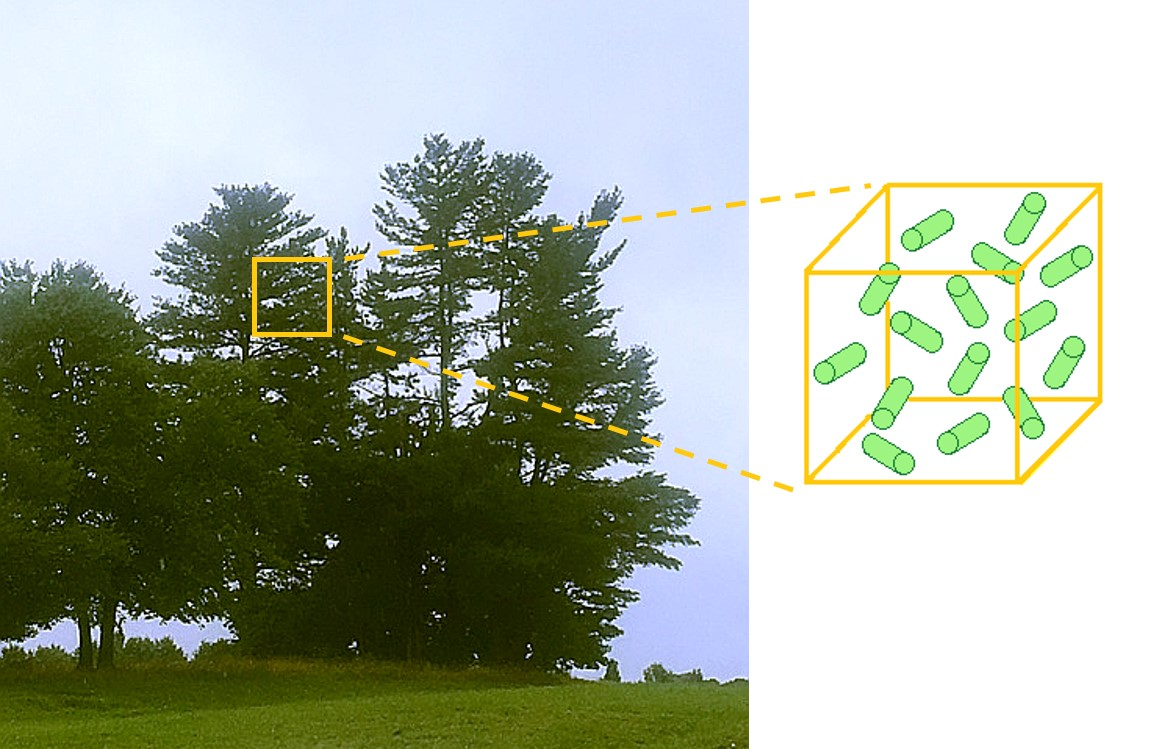
\includegraphics[width=1.0\linewidth]{Picture1.jpg}
	\caption{Vegetation translation to multi-component model}
	\label{fig:Canopymod}
\end{figure}

Equation~(\ref{eq:DragForce}) can be recast in an equivalent form that is more useful for describing vegetation drag~\cite{Mueller2014}:
\begin{equation}
\label{eq:DragForcea}
F  = \frac{\rho}{2} C_{\rm d} \, C_{\mathrm{s}} \, \beta \, \sigma \, U^2
\end{equation}
where $C_{\mathrm{s}}$ is a shape factor defined in this case as the average ratio of the projected area to surface area of the vegetative elements, $\beta$ is the ratio of the volume occupied by vegetation to the volume of the grid cell, $V$, and $\sigma$ is an average surface area to volume ratio of the vegetative elements. Some of the terms are difficult to measure, such as the shape factor and surface to volume ratio, but collectively these terms may be combined to form a parameter that resembles an absorption coefficient:
\begin{equation}
\label{eq:Kappa}
\kappa = C_{\mathrm{s}} \, \beta \, \sigma
\end{equation}
$\kappa$ can be determined by measuring the projected area of light passing a distance $L$ through the vegetation. The relative area of light, or ``free-area coefficient'', is defined by the relation:
\begin{equation}\label{eq:WhiteFraction}
W = {\rm e}^{-\kappa L}
\end{equation}
In the experiments, the cross-section of a small wind tunnel is filled with various amounts and types of vegetation to determine the drag coefficient for the following simplified model:
\begin{equation}\label{eq:Pressure}
F \equiv \frac{\Delta P}{L}  = \frac{\rho}{2} \, C_{\rm d} \, \kappa \, U^2
\end{equation}
\pagebreak


\section{Description of Experiments}
\label{sec:Experiments}


\subsection{Sample Preparation}
\label{ssec:SamplePrep}

The vegetation chosen for this work was a Bakers Blue Spruce ({\em Picea pungens `Bakeri'}), an Evergreen Distylium (Distylium `PIIDIST-I'), a Gold Rider Leyland Cypress ({\em Cupressocyparis leylandii `Gold Rider'}), a Kimberly Queen Fern ({\em Nephrolepis obliterata `Kimberly Queen'}), a Blue Shag Eastern White Pine ({\em Pinus strobus `Blue Shag'}), and a Robin Red Holly ({\em Ilex opaca}). Each sample was chosen based on its local availability. Leaf shapes were varied, including needle, elliptic, scale, and ovate.

The plant samples were cut into 0.5~\si{m} by 0.5~\si{m} by 0.5~\si{m} cubes using a guiding frame (Fig.~\ref{fig:Sampleprep}). The samples completely filled the cross section of the wind tunnel forcing the flow to move through the vegetation as opposed to around it. To easily distinguish the front, back, left, and right side of the cube-shaped vegetation, each side was designated Position A, B, C, or D (Fig.~\ref{fig:Vegpos}). After its initial cut, image analysis, wind tunnel measurements, and water displacement testing were conducted in subsequent order. In some cases, samples were pruned and tested again. In the case of the Bakers Blue Spruce, Gold Rider Leyland Cypress, and Robin Red Holly, four prunings were made with the final one being the removal of all leaves.

\begin{figure} [!]
	\centering 	
	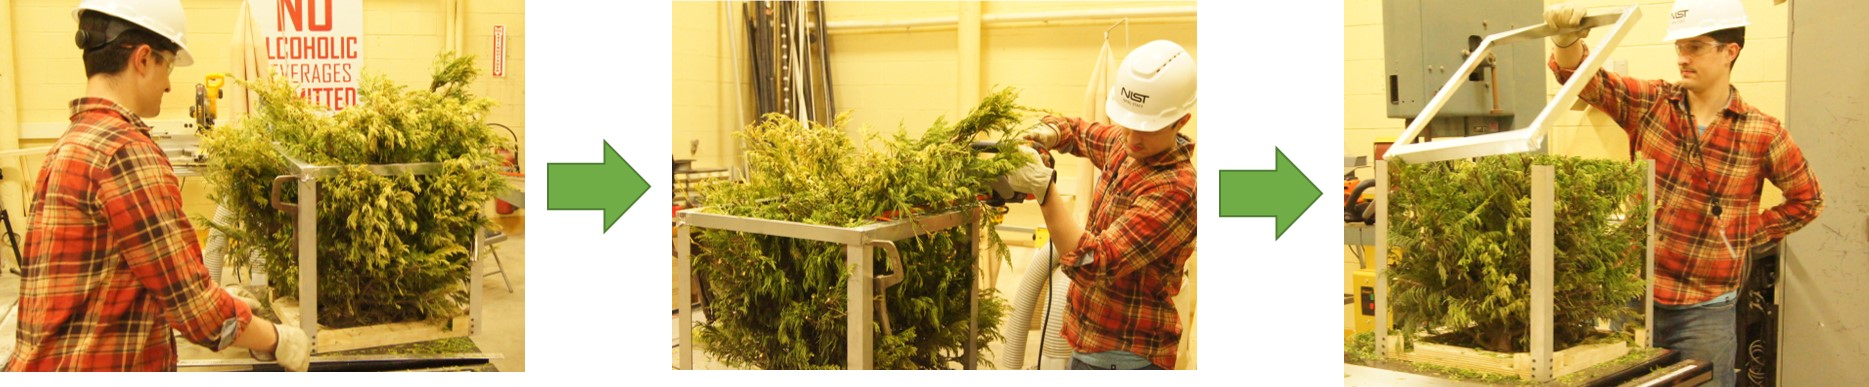
\includegraphics[height=8.in,keepaspectratio]{Picture2.jpg}
	\caption{Cutting procedure of vegetation samples}
	\label{fig:Sampleprep}
\end{figure}
\begin{figure} [!]
	\centering 	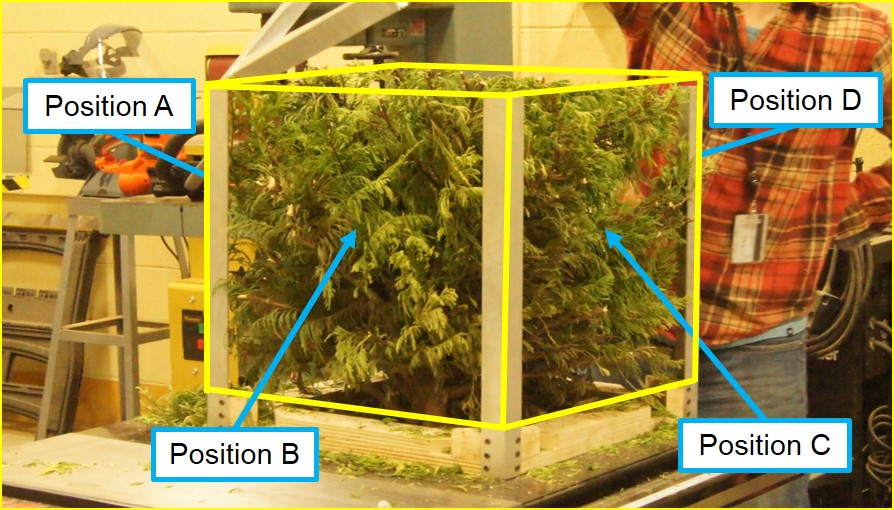
\includegraphics[width=1.0\linewidth]{Picture3.jpg}
	\caption{Prepared vegetation sample's designated orientation}
	\label{fig:Vegpos}
\end{figure}

\subsection{Determining the Free-Area Coefficient via Photography}
\label{ssec:Free-Area Coef. Photo}

The free-area coefficient was determined by placing each vegetation sample on a table located between a large white backdrop and a 0.5~m by 0.5~m cardboard frame, the same dimensions as the tunnel cross section (Fig.~\ref{fig:ImgAnaly}). For each sample cut and position, the projected area was photographed. All images were captured using a Nikon D5600 camera placed on a tripod located approximately 3.6~\si{m} away from the sample. The white backdrop was illuminated using a collection of incandescent and LED lights.

\begin{figure} [!h]
	\centering 	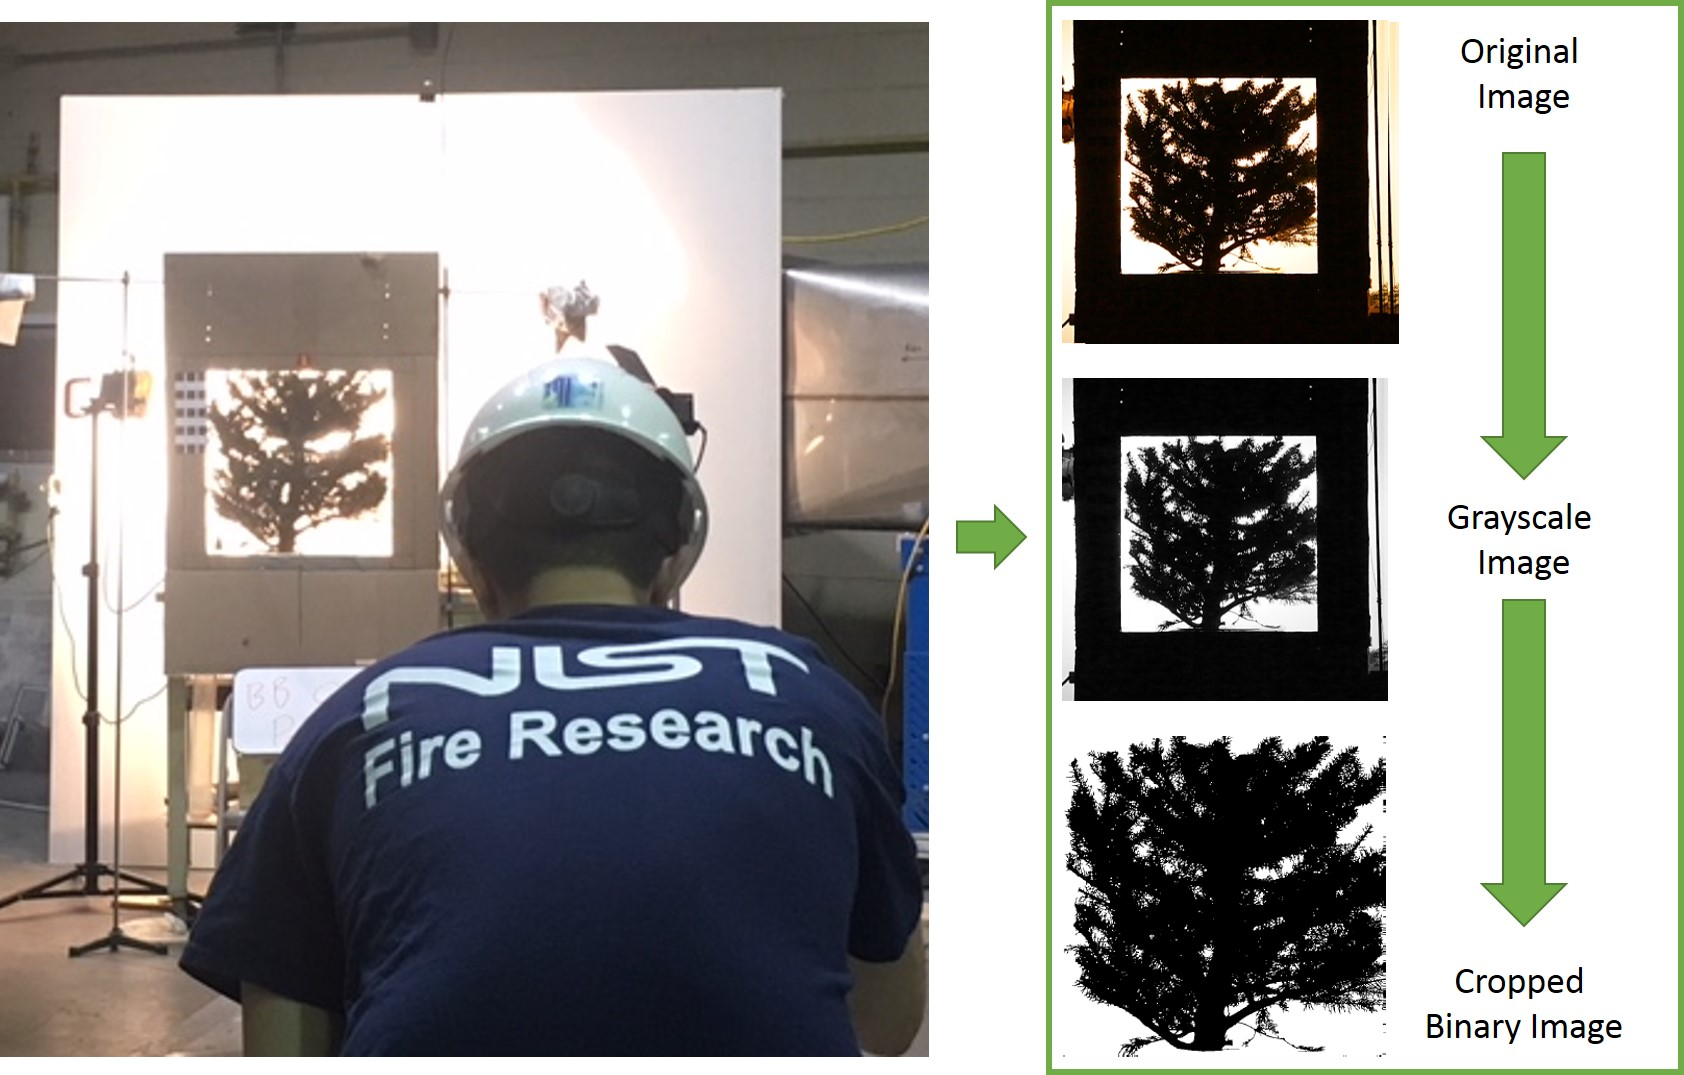
\includegraphics[width=1.0\linewidth]{Picture5.jpg}
	\caption[Setup for photographing vegetation samples]{Setup for photographing vegetation samples (left) and the post-processing procedure for analyzing images (right)}
	\label{fig:ImgAnaly}
\end{figure}

The images were processed using MATLAB's Image Processing Toolbox. Imported colored images were first converted into a grey scale and then a binary (black and white) image using a pre-set threshold level. The binary images were then cropped within the cardboard frame to eliminate non-vegetative substances and to evaluate the projected image of the vegetation exclusively. Once the projected image was obtained, a pixel count was conducted to determine the free-area coefficient of the vegetation, $W$. Once obtained, the free-area coefficient was used to calculate $\kappa$ from Eq.~\ref{eq:WhiteFraction}.

The uncertainty of the free-area coefficient, $W$, is discussed in Appendix~\ref{ssec:FAACUncertainty}.

\subsection{Description of the Wind Tunnel}
\label{ssec:headingscap}

Pressure loss measurements were obtained in a wind tunnel test section with a cross-sectional area of 0.5~\si{m} by 0.5~\si{m} and a length of 2~\si{m}. An image and schematic diagram of the wind tunnel setup is shown in Fig.~\ref{fig:WindtunnelPic}. The volume flow through the tunnel was measured upstream of the vegetation using a Rosemont~485 Annubar~\cite{Annubar}. The pressure drop across the vegetation was measured using an MKS Baratron Type 220D pressure transducer with a range of 0 to 133~Pa (1~torr). The air flow was provided by a 0.91~m axial fan controlled by a variable frequency drive and monitored using the Annubar. Air density was calculated from pressure, temperature, and relative humidity readings of the testing facility. Each sample configuration was subjected to nine different fan speeds ranging from 0 to 88~\% of the full-scale fan speed. The fan speed was not run at full scale due to the risk of exceeding the pressure transducer's pressure limitations. Data was sampled at 90~\si{Hz} for a 30~\si{s} period while maintaining a constant fan speed.

\begin{figure} [!]
	\centering 	
    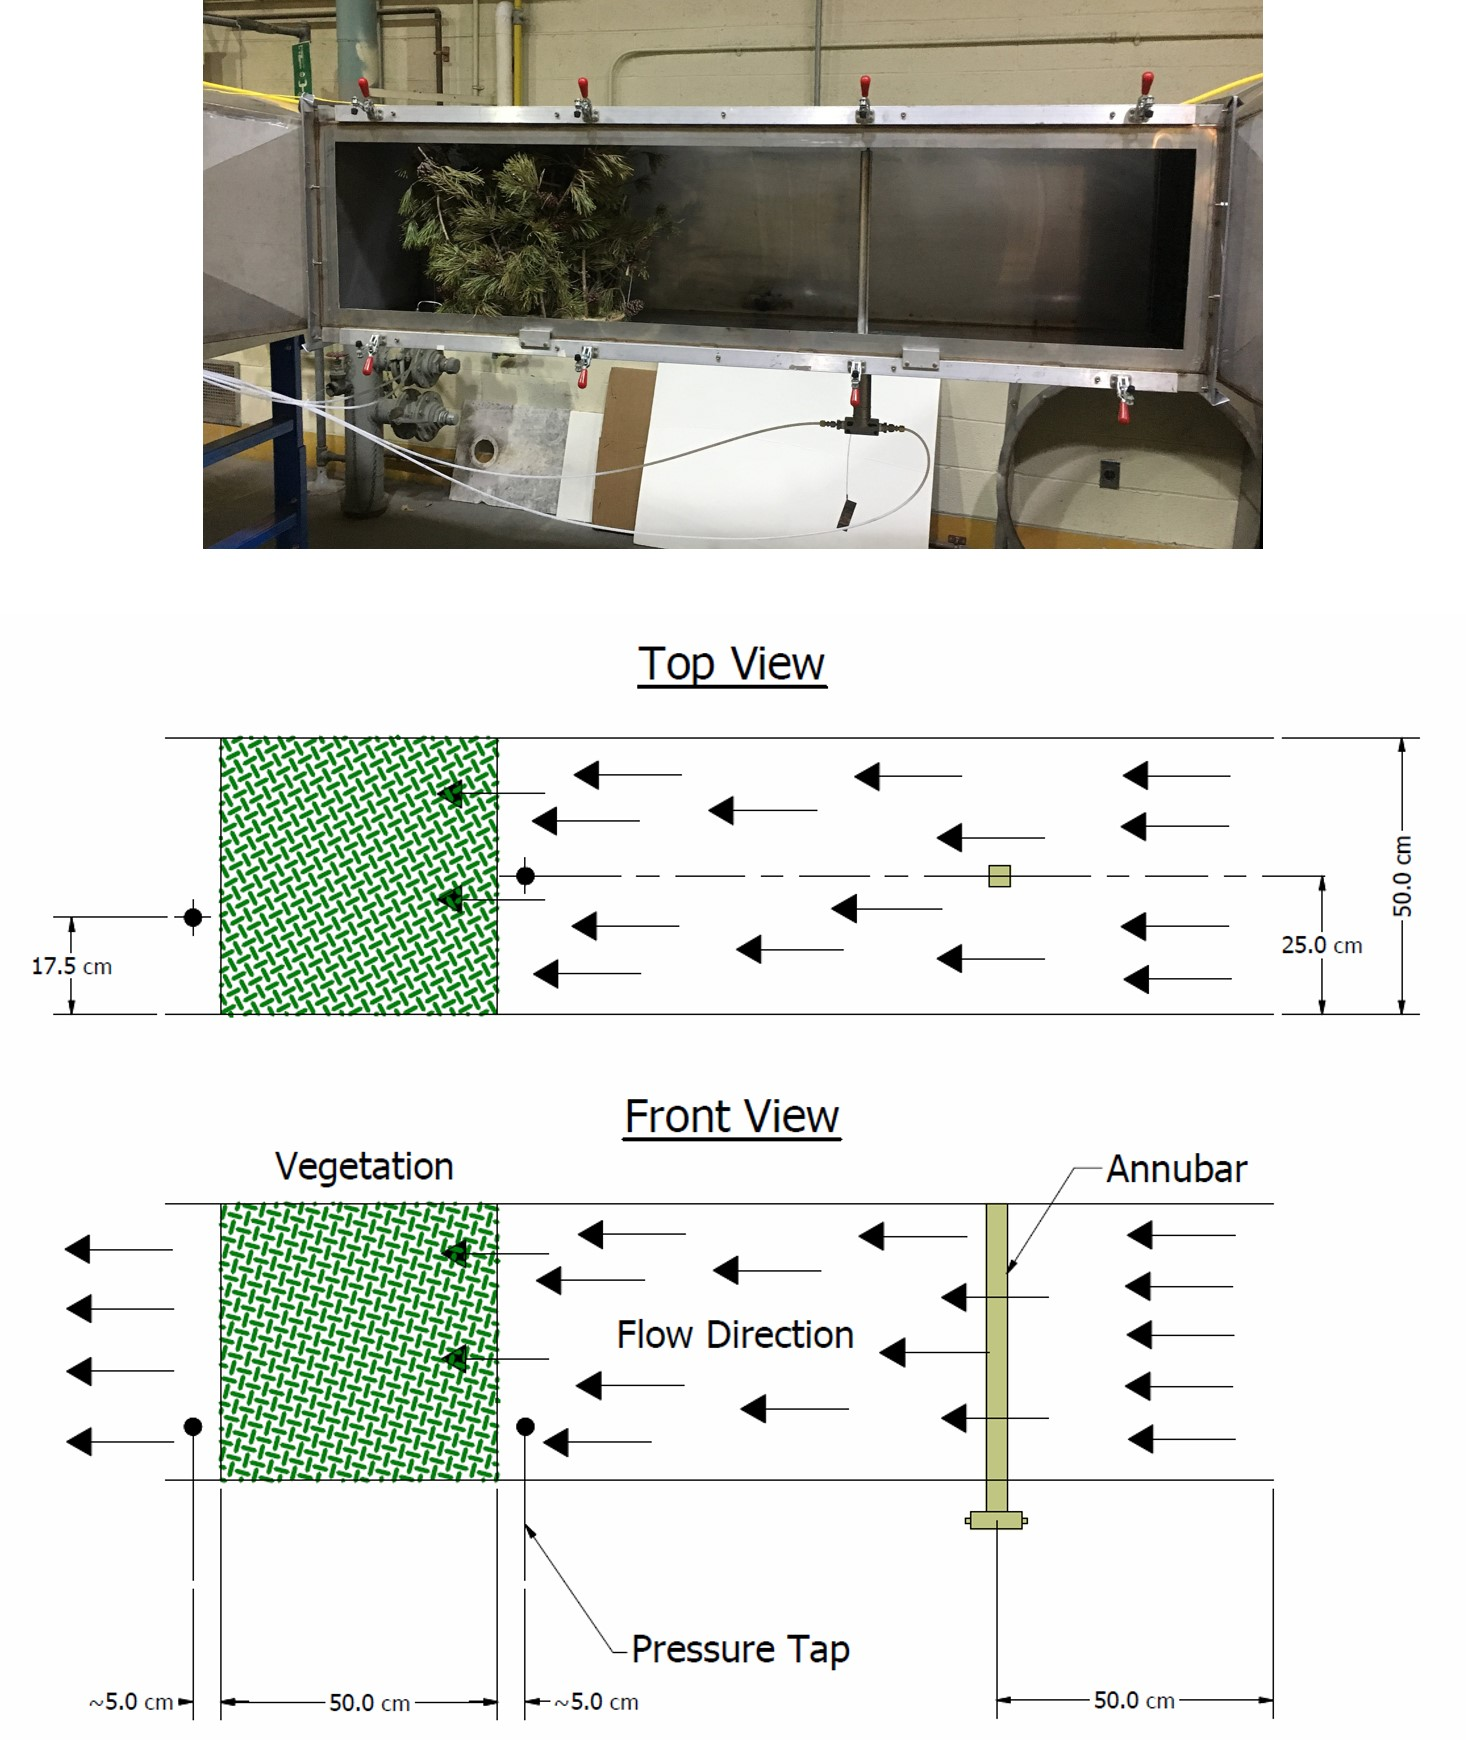
\includegraphics[width=\textwidth,keepaspectratio]{Picture6a.jpg}
	\caption[Wind tunnel experimental setup]{Wind tunnel experimental setup with top and front schematic drawings }
	\label{fig:WindtunnelPic}
\end{figure}

%\begin{figure} [!]
%	\centering 	
%    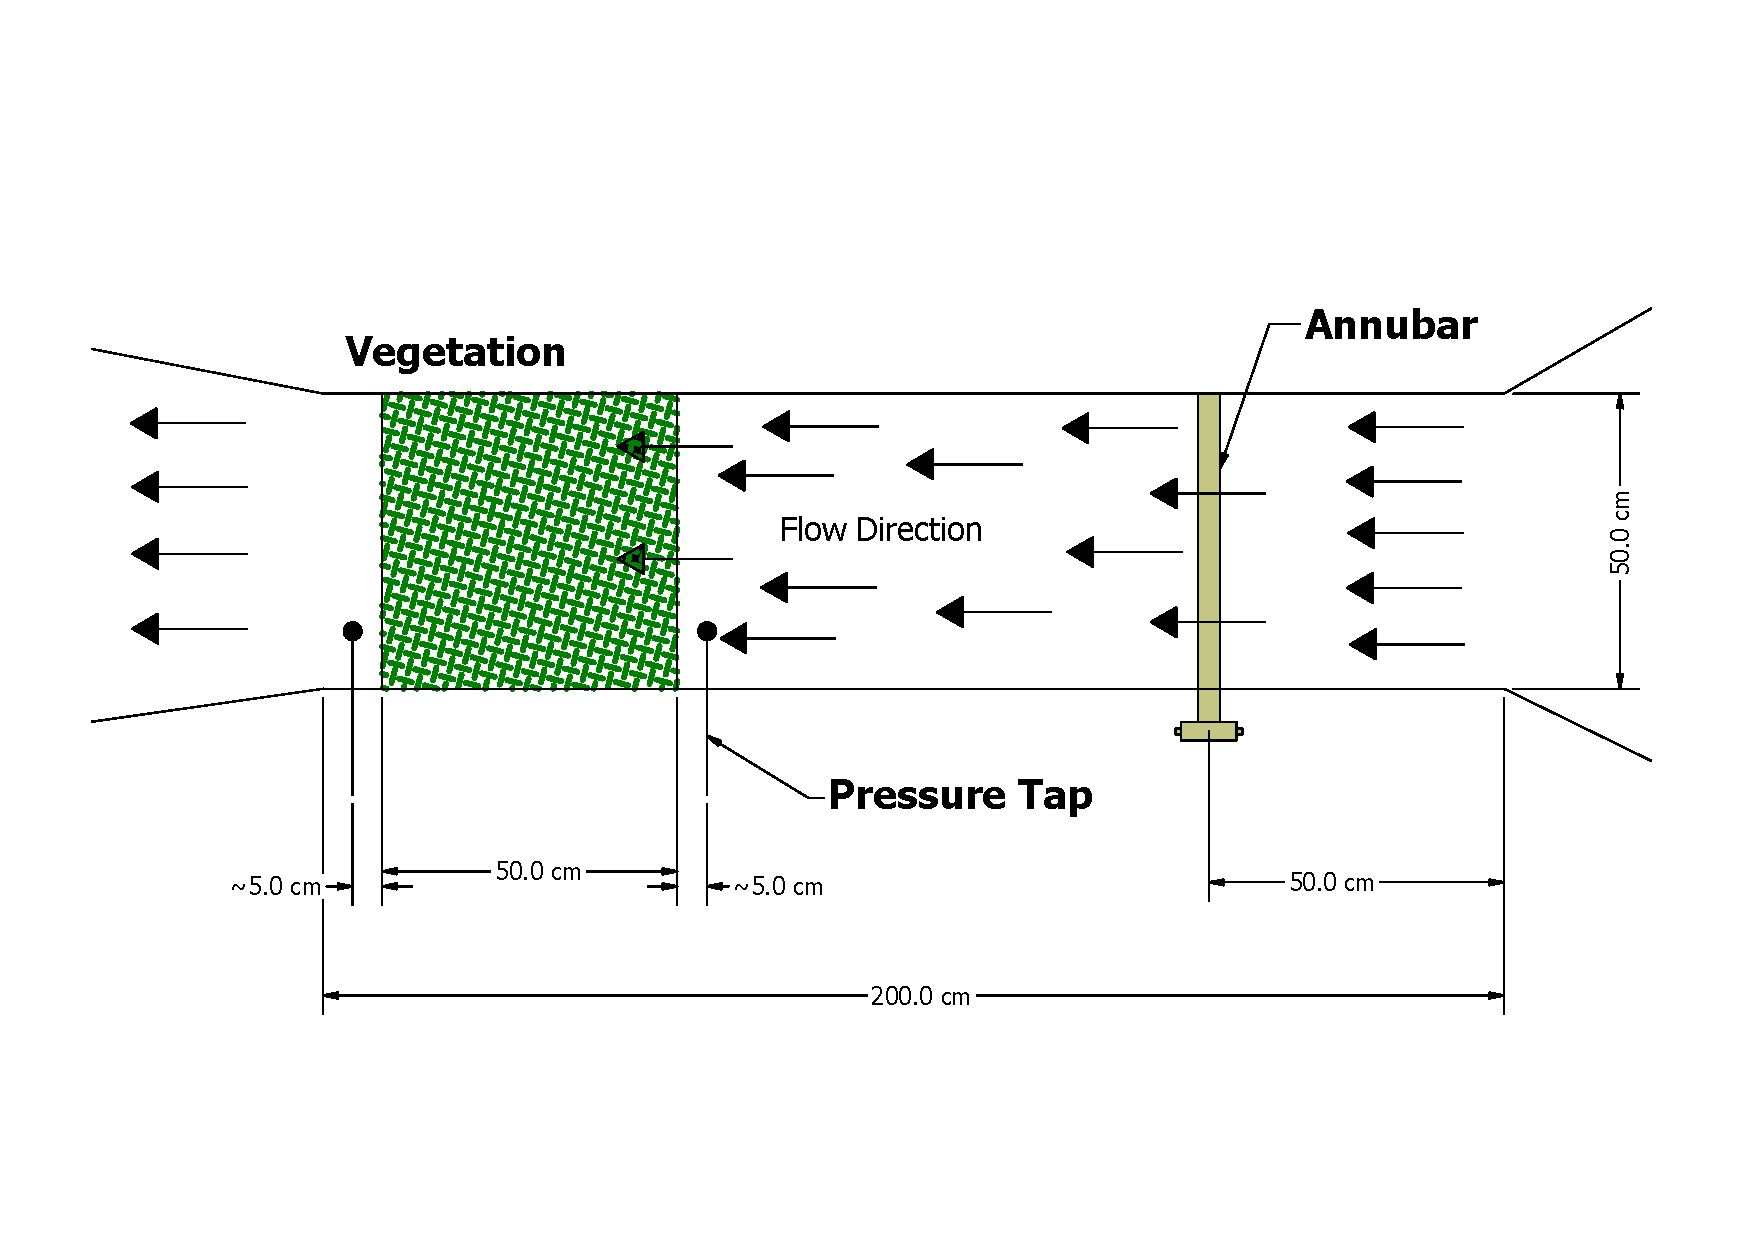
\includegraphics[width=\textwidth,keepaspectratio]{Drawing1.pdf}
%	\caption{Schematic diagram of the wind-tunnel experimental setup}
%	\label{fig:WindtunnelSch}
%\end{figure}

Once a set of measurements was taken at all fan speeds, the wind tunnel was shut off for approximately 5~\si{min}, and then the measurements were repeated. All measurements were repeated three times for each vegetation configuration. The variance homogeneity of the replicate measurements was tested using Hartley's F\textsubscript{max} test. If it was found that the data sets were homogenous, then the measurements were averaged.

An uncertainty analysis was conducted for the pressure and air density measurements and the subsequently determined velocities and drag coefficients. The characterization of the uncertainty for each parameter is provided in Appendix~\ref{sec:UncertaintyDrag}.

\subsection{Determining the Volume of Vegetation via Water Displacement}
\label{ssec:waterdisp}

The volume of the vegetation was measured after a sample cut. The extracted vegetation was separated into branches and leaves and put into cloth mesh bags of known mass and volume, weighed\footnote{The mass was measured to estimate the water absorbed by the sample. The volume of water absorbed was subtracted from the volume of vegetation measured from the beaker.}, and submerged in a bucket. The displaced water flowed through a spout and into a beaker (Fig.~\ref{fig:wdt}). The measurement was repeated three times for each sample. The solid fraction, $\beta$, was calculated by dividing the average sample volume by the volume it occupied (0.5~\si{m} $\times$ 0.5~\si{m} $\times$ 0.5~\si{m} = 0.125~\si{m^{3}}).

The combined standard uncertainty of the measured solid sample volume combines, via quadrature, the Type A standard uncertainty, taken as the standard deviation of the repeated measurements, and the Type~B standard uncertainty, taken as the standard deviation of the assumed uniform distribution that characterizes the uncertainty in the reading of the graduated cylinder, $5/\sqrt{12}$~mL, where the cylinder has 5~mL grading divisions.

\begin{figure} [!]
	\centering 	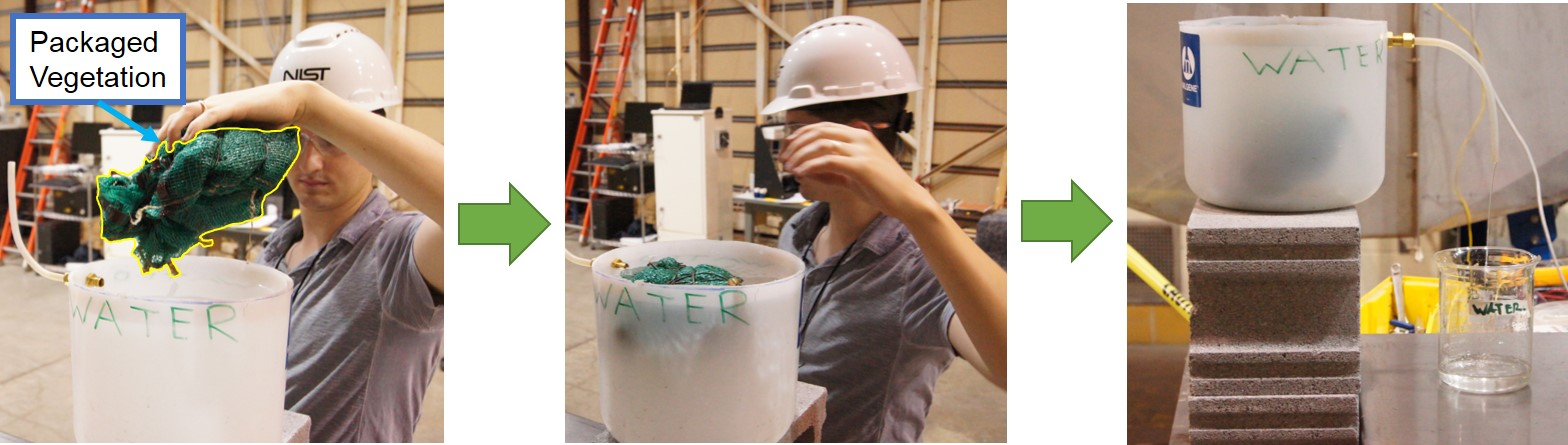
\includegraphics[height=0.95\textheight,keepaspectratio]{Picture7.jpg}
	\caption{Procedure of the water displacement test}
	\label{fig:wdt}
\end{figure}

\pagebreak



\section{Results}
\label{sec:results}

The key results of this work are the relationship between the ``absorption coefficient,'' $\kappa$, and the solid fraction, $\beta$, and more importantly the drag coefficient derived from the wind tunnel measurements.

\subsection{Relationship between the absorption coefficient $\kappa$ and solid fraction $\beta$ }

Figure~\ref{fig:betavkappa} presents the relationship between the averaged ``absorption coefficient,'' $\kappa$, and the solid fraction, $\beta$, for the sample configurations of the Bakers Blue Spruce, Evergreen Distylium, Gold Rider Leyland Cypress, and Robin Red Holly . The symbols indicate the measured values while the dotted lines represent a linear regression fit. Each line represents a particular type of vegetation that has been pruned, reducing both the volume fraction, $\beta$, the projected free-area coefficient, $W$, and the corresponding value of $\kappa$. There ought to be a linear relationship between $\kappa$ and $\beta$ if the shape factor, $C_{\rm s}$, and surface to volume ratio, $\sigma$ are constant, as shown in Eq.~(\ref{eq:Kappa}). However, this is not the case when the vegetative components are not uniform in size. Take, for example, the Robin Red Holly data shown in Fig.~\ref{fig:betavkappa}. As $\beta$ decreases, $\kappa$ should approach zero, as demonstrated by most samples. As the leaves of the Robin Red Holly were pruned, $\kappa$ decreased significantly even though its volume fraction did not, owing to the fact the ratio of branch to leaf volume of the Robin Red Holly is substantially higher than the other plant species, as shown in Table~\ref{tab:RatioTable}.  As a result, the free-surface area, $W$, decreases from the removal of leaves, thus reducing $\kappa$, while still maintaining a relatively consistent solid fraction due to the significant volume contribution of the branches.

\begin{figure}[!h]
	\centering 	
    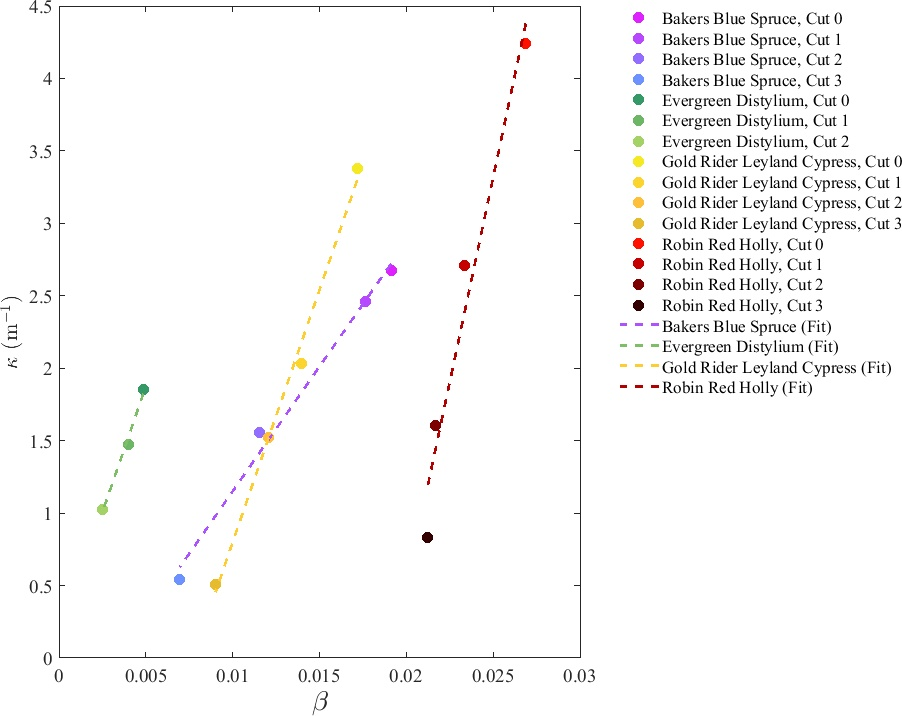
\includegraphics[width=1\linewidth]{Picture12.jpg}
	\caption[Comparison of ``absorption coefficient,'' $\kappa$, and solid fraction, $\beta$]{Calculated ``absorption coefficient'' ($\kappa$) of vegetation sample configuration plotted against the corresponding solid fractions ($\beta$)}
	\label{fig:betavkappa}
\end{figure}



\begin{table}[!h]
\caption[Branch and leaf volume ratio of vegetation samples]{Branch and leaf volume ratio of vegetation samples with mulitple cut iterations}
\label{tab:RatioTable}
\centering
	
	\begin{tabular*}{\textwidth}{lcclcc}	
			\hline
\rule{0pt}{14pt}\textbf{Sample}	&\textbf{$\beta$\,(\%)}	& {\bf Branch/Leaf Vol.}  \hspace{.2in}  		&\textbf{Sample}		&	\textbf{$\beta$\,(\%)}	& {\bf Branch/Leaf Vol.}	\\
\hline
\\[0.01cm]
Blue Spruce		    		&	1.9			& 	1.1			        				& Cypress       		&	1.7		&	1.5						\\
					&	1.8			& 	1.3							&				&	1.4		&	2.2						\\
					&	1.2			& 	1.5							&				&	1.2		&	3.0						\\
					&	0.7			&	N/A							&				&	0.9		&  	N/A 						\\
					&				&								&				&			&       							\\
Distylium				&	0.5			&	1.0							& Red Holly	     		&	2.7		&	11						\\
					&	0.4			&	1.4							&				&	2.3		&	16						\\
					&	0.3			&	3.3							&				&	2.2		&	47						\\
					&				&								&				&	2.1		&        N/A 						\\
\\[0.005cm]
\hline														

\end{tabular*}
\end{table}

\pagebreak


\subsection{Vegetation Canopy Drag Coefficients}
\label{ssec:headingscap}

Figure~\ref{fig:DPvU(Overall)} displays the relationship between the freestream velocity and the pressure drop for each sample configuration. The results demonstrate the expected quadratic relationship. Replotting the data as shown in Fig.~\ref{fig:DPoveraf(Overall)} yields the drag coefficient for each sample configuration as determined by calculating the slope of each line of data points. No linear regression fitting was observed to have a coefficient of determination less than 0.98, indicating a close representation of the fitted regression line to the measured data. A summary of all 68 calculated drag coefficients and their respective uncertainties are presented in Table \ref{tab:SumTable}\footnote{The procedure for determining the drag coefficient uncertainty as shown in this table can be found in Appendix~\ref{sec:UncertaintyDrag}. For most instances, the uncertainty in the velocity measurement was found to be the primary contributor to the drag coefficient uncertainty. In other cases, the uncertainty of the measured pressure loss across the vegetation was the primary contributor to the drag coefficient uncertainty.}.

\begin{sidewaysfigure} [!]
	\centering
	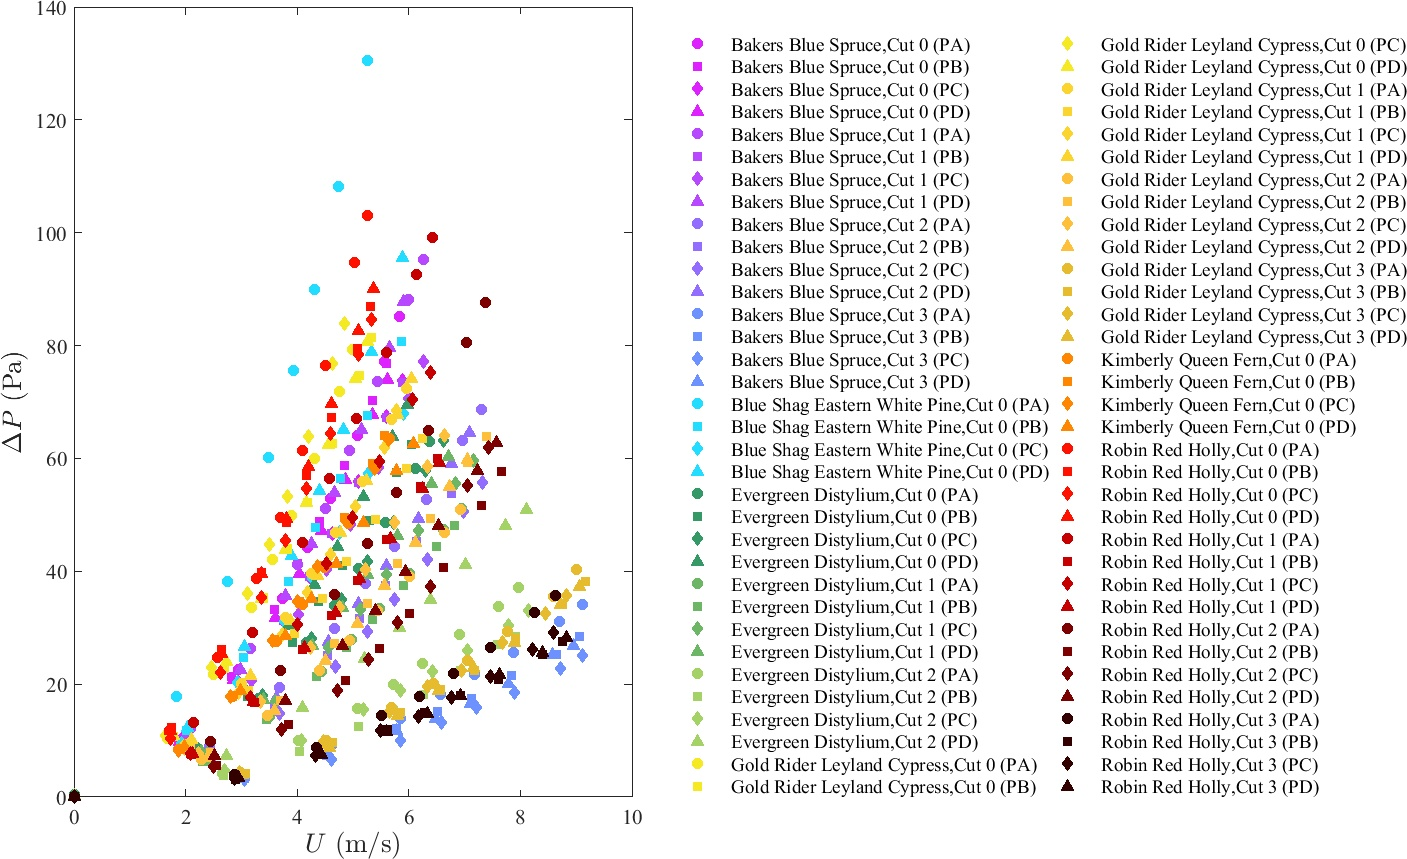
\includegraphics[width=\textwidth,keepaspectratio]{Picture8.jpg}
	\caption[Differential pressure measurements of vegetation samples]{Differential pressure measurements of vegetation samples subjected to a range of freestream velocities}
	\label{fig:DPvU(Overall)}
\end{sidewaysfigure}

\begin{sidewaysfigure}[!]
	\centering
	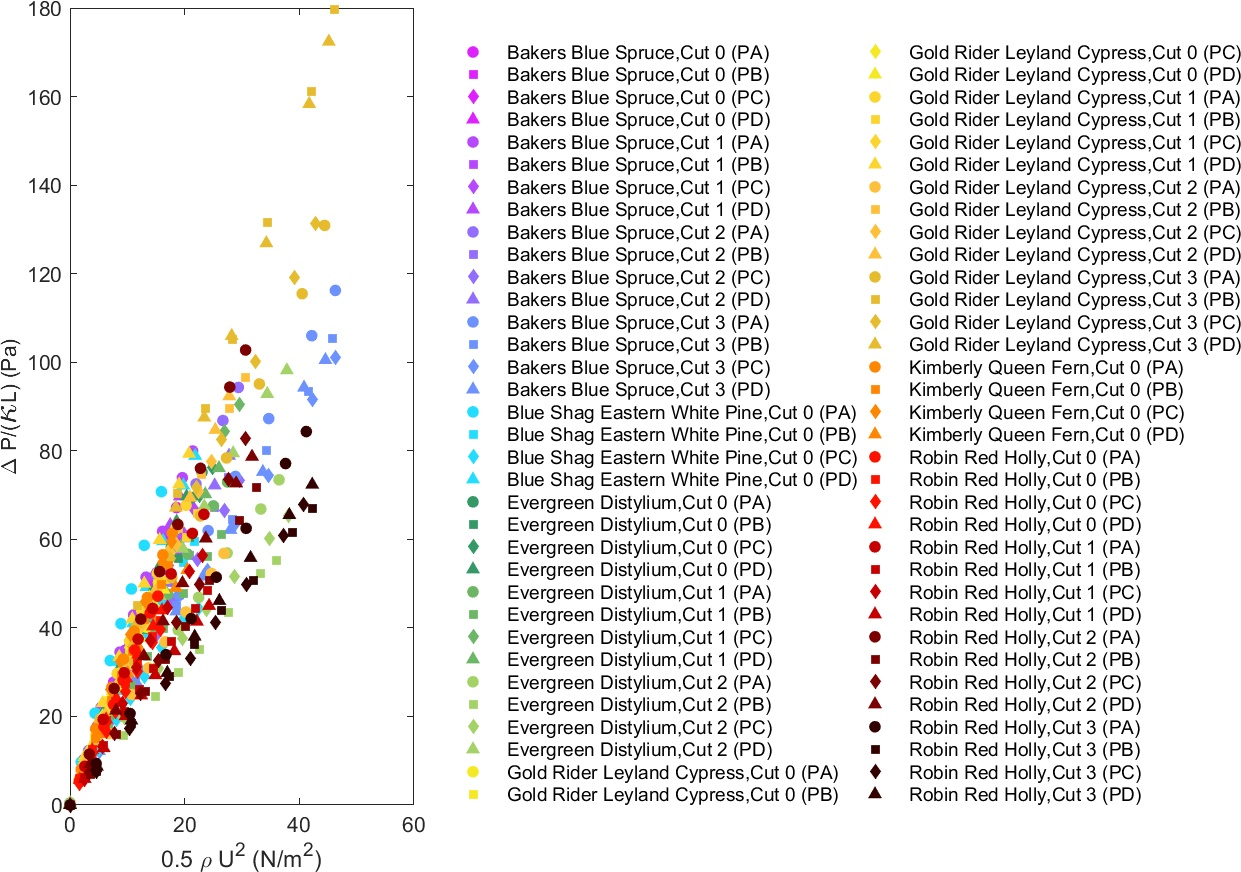
\includegraphics[width=\textwidth,keepaspectratio]{Picture9.jpg}
	\caption{Differential pressure measurements of vegetation samples over ($\kappa \, L$) vs. dynamic pressure}
	\label{fig:DPoveraf(Overall)}
\end{sidewaysfigure}

The distribution of the measured drag coefficients for all sample configurations is shown in Fig.~\ref{fig:Histogram}. The collection of sample configurations is divided into two groups based on leaf shape (i.e., narrow and broad). The narrow leaves group included the Bakers Blue Spruce, Blue Shag Eastern White Pine, and Gold Rider Leyland Cypress while the broad leaves group was comprised of the remaining species. The average drag coefficient of all sample configurations was determined to be 2.8 with an expanded uncertainty of 0.4.

\begin{figure}[!]
	%\centering 	
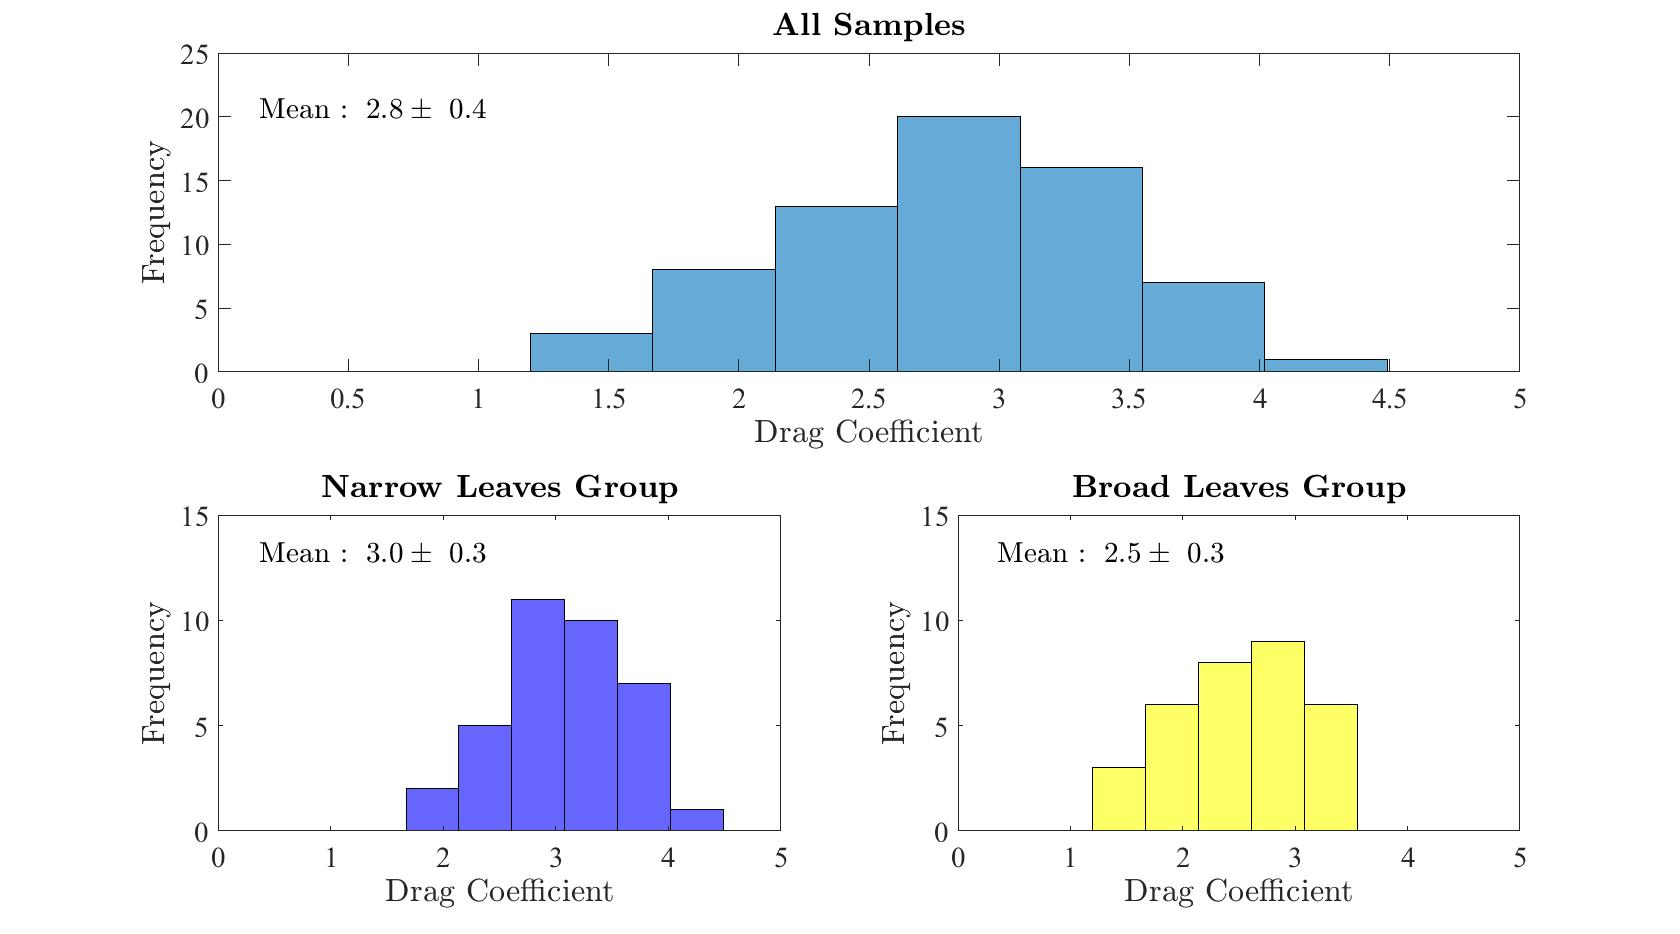
\includegraphics[width=\textwidth,keepaspectratio]{Picture11.jpg}
	\caption[Distribution of drag coefficients for all samples (top), samples with narrow leaves (bottom left), samples with broad leaves (bottom right)]{Distribution of vegetation samples drag coefficients with noted mean and standard deviation values}
	\label{fig:Histogram}
\end{figure}

To determine if the average drag coefficient depends on the type of vegetation a random effects one-way ANOVA\footnote{Analysis of Variance} was implemented on the drag coefficients of the different vegetation samples. The analysis yielded a significant variation ($F(5,62)=4.88$, $p=7.97 \times 10^{-4}$) among the species\footnote{The $F$ refers to the statistic obtained from the F-test conducted in the ANOVA, the 5 and 62 in brackets represent the degrees of freedom, and the 4.88 is the actual F statistic derived from the ANOVA. The $p$ refers to the significance level determined from the F statistic and the $7.97 \times 10^{-4}$ is the actual p-value which was determined to be less than the chosen confidence level of 0.05, indicating a significant difference between the mean drag coefficients of the samples.}. A Tukey's test~\cite{Lane2010} was subsequently applied to determine if the species-specific average drag coefficients were significantly different from each other. The results showed one significant difference between the species' average drag coefficients: the Robin Red Holly and Gold-Rider Leyland Cypress. Despite the significant difference, the average drag coefficients of these two plant species are still within the uncertainty bound of the overall drag coefficient and therefore are not large enough to have a practical implication.

Further analysis was conducted to compare the two leaf shape groups. A one-way random effects model~\cite{Toman2009} for the measurements of the narrow leaves group assumes that the drag coefficients are normally distributed:
\begin{equation}
\label{eq:NarrowLeavesDragCoefficient}
C_{\rm d,ij}\sim\,N(m_{1},{u_{ij}}^2+{\sigma_1}^2),\, i=\, 1,...,3; j=\, 1,...,n_{i}
\end{equation}
where $i$ denotes the plant species (1 for Bakers Blue Spruce, 2 for Blue Shag Eastern White Pine, and 3 for Gold Rider Leyland Cypress), and $j$ denotes the specific configuration of the plant in the tunnel. The sample size for a given plant species is $n_{i}$. The value of $u_{ij}$ is the standard uncertainty of the measured drag coefficient for a specific species and configuration. The parameters $m_{1}$ and $\sigma_1$ are the mean and standard deviation for the narrow leaves group, respectively. The drag measurements of the broad leaves group are modeled in a similar way:
\begin{equation}
\label{eq:BroadLeavesDragCoefficient}
C_{\rm d,ij}\sim\,N(m_{2},{u_{ij}}^2+{\sigma_2}^2),\, i=\, 4,...,6; j = 1,...,n_{i}
\end{equation}
where $i$\,=\,4 for Distylium, $i$\,=\,5 for Fern, and $i$\,=\,6 for Red Holly). The parameters $m_2$ and $\sigma_2$ are the mean and standard deviation for the broad leaves group, respectively.

Using a Bayesian statistical model~\cite{Gelman2008} with non-informative priors for $m_{1}$, $m_{2}$, $\sigma_1$, and $\sigma_2$, we obtain via Markov Chain Monte Carlo implemented in OpenBUGS~\cite{Lunn2009} the posterior means and standard uncertainties of the parameters. These are: $m_{1}$ is 3.0 with an expanded (95~\%) uncertainty of 0.3, $m_{2}$ is 2.5 with an expanded (95~\%) uncertainty of 0.3, and the 95~\% uncertainty interval for the difference $m_{1}-m_{2}$ is (0.052, 0.87). This may be interpreted as a rejection of a hypothesis test of $H_{0}$:\,$m_{1}-m_{2}$=\,0 at a level of 5~\%. Despite the differences in the average drag coefficients of both groups, they both lie within the uncertainty bound of the overall average drag coefficient, which suggests that mean drag coefficient obtained from all samples could be a reasonable approximation when applied as a consistent drag coefficient for vegetation canopies in CFD models.

\begin{table}[!]

\caption{Drag Coefficient Summary of Vegetation Samples.}
\label{tab:SumTable}
\centering
	\footnotesize
	\begin{tabular}{cccccccccccc}	
			\hline
\textbf{Sample}		& \textbf{$\beta$\,(\%)}		&\textbf{Position}& $C_{\rm d}$ &\textbf{Uncertainty}	&\textbf{Sample}		& \textbf{$\beta$\,(\%)}&\textbf{Position}& 	\textbf{$C_{\rm d}$ }&\textbf{Uncertainty}\\
\hline
\\[0.05cm]
Blue Spruce			&	1.9	&	A	& 	3.6		&	0.5			& Cypress       		&	1.7	&	A	& 	3.0	&	0.5	\\
				&		&	B	& 	3.1		&	0.5			&				&		&	B	& 	3.2	&	0.5	\\
				&		&	C	& 	3.1		&	0.4			&				&		&	C	& 	3.4	&	0.5	\\
				&		&	D	& 	3.0		&	0.4			&				&		&	D	& 	3.0	&	0.4	\\
				&	1.8	&	A	& 	3.8		&	0.5			&				&	1.4	&	A	& 	3.3	&	0.4	\\
				&		&	B	& 	3.0		&	0.4			&				&		&	B	& 	2.9	&	0.4	\\
				&		&	C	& 	3.1		&	0.4			&				&		&	C	& 	3.3	&	0.4	\\
				&		&	D	& 	3.6		&	0.4			&				&		&	D	& 	3.8	&	0.4	\\
				&	1.2	&	A	& 	3.2		&	0.4			&				&	1.2	&	A	& 	2.1	&	0.5	\\
				&		&	B	& 	2.6		&	0.3			&				&		&	B	& 	3.2	&	0.3	\\
				&		&	C	& 	2.5		&	0.3			&				&		&	C	& 	3.1	&	0.4	\\
				&		&	D	& 	2.8		&	0.3			&				&		&	D	& 	3.3	&	0.4	\\
				&	0.7	&	A	& 	2.5		&	0.4			&				&	0.9	&	A	& 	2.9	&	0.4	\\
				&		&	B	& 	2.3		&	0.4			&				&		&	B	& 	3.9	&	0.4	\\
				&		&	C	& 	2.2		&	0.4			&				&		&	C	& 	3.0	&	0.5	\\
				&		&	D	& 	2.2		&	0.4			&				&		&	D	& 	3.8	&	0.5	\\
				&		&		& 			&				&				&		&		& 		&		\\
White Pine	       		&	2.8	&	A	& 	4.4		&	0.7			& Fern	       		&	0.4	&	A	& 	3.4	&	0.5	\\
				&		&	B	& 	2.8		&	0.4			&				&		&	B	& 	3.1	&	0.4	\\	
				&		&	C	& 	2.1		&	0.4			&				&		&	C	& 	3.3	&	0.5	\\
				&		&	D	& 	3.6		&	0.5			&				&		&	D	& 	2.6	&	0.4	\\
				&		&		& 			&				&				&		&		& 		&		\\
Distylium			&	0.5	&	A	& 	3.2		&	0.4			&Red Holly			&	2.7	&	A	& 	3.1	&	0.5	\\
				&		&	B	& 	2.9		&	0.4			&				&		&	B	& 	2.6	&	0.4	\\
				&		&	C	& 	3.1		&	0.4			&				&		&	C	& 	2.5	&	0.4	\\
				&		&	D	& 	3.4		&	0.4			&				&		&	D	& 	2.7	&	0.4	\\
				&	0.4	&	A	& 	2.7		&	0.3			&				&	2.3	&	A	& 	2.8	&	0.4	\\
				&		&	B	& 	2.3		&	0.3			&				&		&	B	& 	2.0	&	0.3	\\
				&		&	C	& 	3.1		&	0.4			&				&		&	C	& 	2.5	&	0.3	\\
				&		&	D	& 	2.9		&	0.4			&				&		&	D	& 	1.8	&	0.3	\\
				&	0.3	&	A	& 	2.0		&	0.3			&				&	2.2	&	A	& 	3.4	&	0.3	\\
				&		&	B	& 	1.5		&	0.2			&				&		&	B	& 	2.2	&	0.2	\\
				&		&	C	& 	1.7		&	0.3			&				&		&	C	& 	2.7	&	0.3	\\
				&		&	D	& 	2.6		&	0.3			&				&		&	D	& 	2.5	&	0.3	\\
				&		&		& 			&				&				&	2.1	&	A	& 	2.1	&	0.3	\\	
				&		&		& 			&				&				&		&	B	& 	1.6	&	0.3	\\
				&		&		& 			&				&				&		&	C	& 	1.6	&	0.3	\\
				&		&		& 			&				&				&		&	D	& 	1.7	&	0.3	\\
\\[0.05cm]
\hline														
\end{tabular}
\end{table}

\section{Comparison Between Vegetation Data and Tube Bank Models}
\label{sec:comp}

In comparison to previous work~\cite{Cao2012,Jalonen2014,Mayhead1973,Gillies2002,Ishikawa2006}, the magnitude of the measured drag coefficients in this study is relatively large. As discussed in Section~\ref{sec:intro}, most previous studies have measured the wind resistance of a single plant or tree within a larger wind tunnel while this work considered a relatively homogenous distribution of vegetation within a tunnel. The interpretation of ``freestream'' velocity, shape factor, cross-sectional area, and so on, are often different in these studies, making it difficult to compare drag coefficients from one study to another. Within the field, there is no single definition of drag coefficient regarding vegetation.

As a way to verify the accuracy of our wind tunnel measurements and the validity of our drag coefficient derivation, we considered a bank of regularly-spaced, staggered, vertical cylinders within our wind tunnel, using both actual steel rods and empirical results from Idelchik~\cite{Idelchik1994}. For each of the measured vegetation samples, a comparable configuration of vertical tubes was chosen such that the volume fraction, $\beta$, ``absorption coefficient,'' $\kappa$, and characteristic diameter, $D$, match as closely as possible (see Table~\ref{tab:tube_parameters}). The characteristic diameter was calculated from Eq.~\ref{eq:Kappa} using the measured $\beta$ and $\kappa$ values and assuming a cylindrical shape factor ($C_{\mathrm{s}} = 1/\pi$). To account for the repeated tube formation for each row the $\kappa$ value of the tube bank was determined from the distance between rows, $L'$, and Eq.~\ref{eq:WhiteFraction}. According to Idelchik, the expected pressure drop through the tube bank is:
\begin{equation}
\label{eq:IdelchickTB}
\Delta P = \frac{\rho}{2}\, \zeta  \left( \frac{U}{W} \right)^2  \quad ; \quad \zeta = A \, \mathrm{Re}^{-0.27} (N_\mathrm{r}+1) \quad ; \quad  \mathrm{Re} = \frac{(U/W) \, D \, \rho}{\mu_\mathrm{air}}
\end{equation}
where $A$ is a geometric parameter determined from the tube bank configuration, $N_\mathrm{r}$ is the number of rows of tubes, $U/W$ is the average velocity of air flowing through the tubes, and Re is the Reynolds number which must be greater than 3000 for the empirical model to apply. Setting the pressure drop, $\Delta P$, in Eq.~(\ref{eq:IdelchickTB}) equal to that in Eq.~(\ref{eq:Pressure}) leads to an equivalent drag coefficient for the tube bank:
\begin{equation}
   C_\mathrm{d} = \frac{\zeta/W^2}{\kappa \, L}
\end{equation}

\begin{table}[!]
    \centering
    \caption{Parameters used in comparing vegetation with a comparable tube bank configuration}
    \label{tab:tube_parameters}
    \begin{tabular}{|c|c|c|c|c|c|c|c|c|c|}
    \hline
                                 & \multicolumn{2}{|c|}{$\beta$ (\%)} & \multicolumn{2}{|c|}{$\kappa$ (m$^{-1}$)} & \multicolumn{2}{|c|}{$D$ (mm)} &                             &                         &         \\ \cline{2-7}
    \raisebox{1.5ex}[0pt]{Pos.}  & Veg.             & Tubes      & Veg.                 & Tubes              & Veg.              & Tubes      & \raisebox{1.5ex}[0pt]{Rows} & \raisebox{1.5ex}[0pt]{$\textfrac{\rm{Tubes}}{\rm{Row}}$} &\raisebox{1.5ex}[0pt]{$L'$ (cm)}\\ \hline \hline
    \multicolumn{10}{|c|}{Blue Spruce}                                                                                                                                                    \\ \hline
    A                            & 1.8            & 1.8      & 2.4                  & 2.4                & 9.4               & 10.6        & 5                           & 10           &          10.0           \\ \hline
    B                            & 1.8            &1.8     & 2.6                & 2.6               &8.6               & 9.5       & 7                           & 9                      &         7.1  \\ \hline
    C                            & 1.8            & 1.7      & 2.3                  & 2.3                & 9.7               & 11.2       &4                            & 11            &      12.5             \\ \hline
    D                            & 1.8           & 1.8      & 2.5                 & 2.5               & 8.9             & 10.4       & 4                           & 13                 &  12.5             \\ \hline
        \multicolumn{10}{|c|}{Cypress}                                                                                                                                                    \\ \hline
    A                            &1.4           & 1.4      & 2.1                  & 2.2                & 8.3              & 8.9       & 7                           & 8                 &   7.1         \\ \hline
    B                            & 1.4          & 1.4      & 1.9                  & 2.0               & 9.2               & 10.7        & 3                           & 13            &   16.7                 \\ \hline
    C                            & 1.4           & 1.4     & 2.2                  & 2.2                & 8.1               & 9.3       & 4                          & 13               &   12.5       \\ \hline
    D                            & 1.4            & 1.4      & 1.9                  & 1.9                & 9.4               & 10.2       & 6                          & 7              &   8.3             \\ \hline
    \end{tabular}
\end{table}

\begin{figure}[!]
	\centering 	
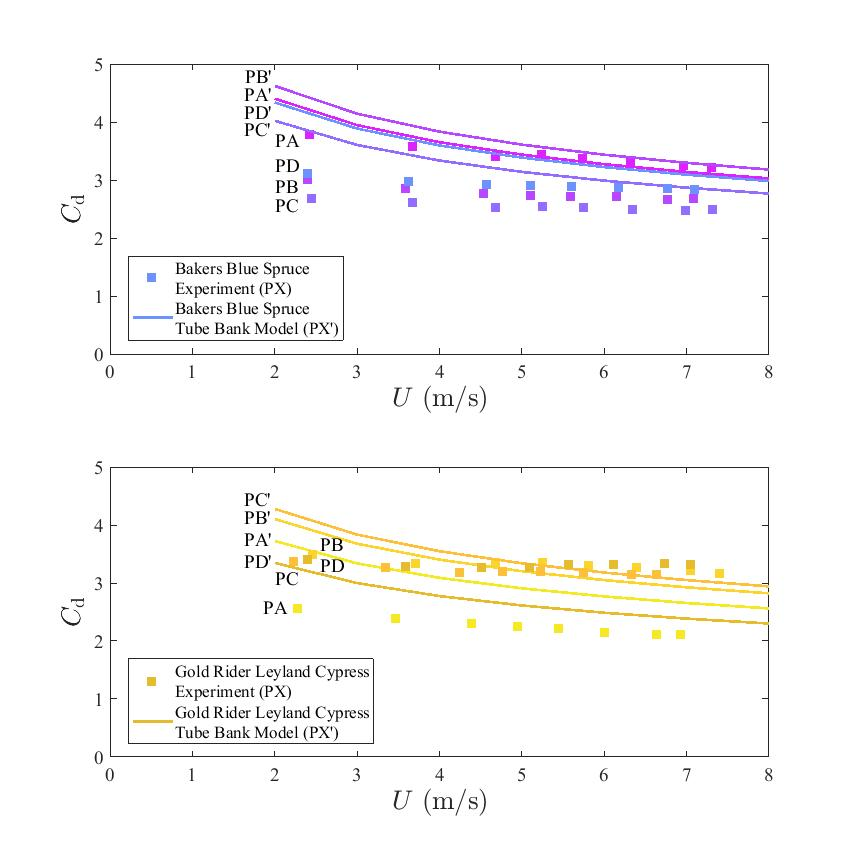
\includegraphics[width=\textwidth,keepaspectratio]{Picture13.jpg}
	\caption[Drag Coefficient comparison between vegetation samples and tube bank configurations]{Drag Coefficient comparison between vegetation sample configurations [Bakers Blue Spruce ($\beta$=1.8\%) and Gold Rider Leyland Cypress ($\beta$=1.4\%)] and their corresponding tube bank configuration with respect to velocity}
	\label{fig:TBGR}
\end{figure}

Figure~\ref{fig:TBGR} compares the drag coefficients from the Gold Rider Leyland Cypress and Bakers Blue Spruce with their tube bank equivalents. While the match is not expected to be perfect given the difference in skin fraction, shape, and so on, the drag coefficient of each configuration is comparable.
\pagebreak

\section{Conclusion}

This report documents a series of experiments implemented to determine the absorption coefficient, pressure loss, and the solid fraction of different types of vegetation sample configurations. The primary objective of this work was to calculate the drag coefficients of ``bulk'' vegetation that can be incorporated into CFD models. In addition to establishing drag coefficients of ``bulk''  vegetation, notable findings regarding vegetation structure and similarities between drag coefficients of plant species were also discovered from this work. It cannot be concluded, however, that the findings from this work applies to all ``bulk'' vegetation, but exclusively to the samples studied in these experiments.

\begin{enumerate}
  \item The calculated absorption coefficient for each sample demonstrated a strong relationship with its corresponding solid fraction.
  \item The overall average drag coefficient of the bulk vegetation was found to be 2.8 with an expanded uncertainty of 0.4. The differences between the average drag coefficients of different plant species as well as the leaf type groups were shown to be significant, while still falling in the overall mean's uncertainty bound, suggesting that the overall average drag coefficient could be used as a constant value in CFD models of various plant types.
\end{enumerate}

\section*{Acknowledgments}

\noindent Matthew Bundy and Artur Chernovksy of the National Fire Research Laboratory assisted in conducting these experiments and in processing the data.   \\
%%%%%%%%%%%%%%%%%%%%%%%%%%%%%%%%%%%%%%%%%%%%%%%%%%%%%%%%%%%%%%%%%%%%
%   Acknowledgments not required
%%%%%%%%%%%%%%%%%%%%%%%%%%%%%%%%%%%%%%%%%%%%%%%%%%%%%%%%%%%%%%%%%%%%
\pagebreak
\section*{References}
\addcontentsline{toc}{section}{References}
\bibliographystyle{unsrt}
\bibliography{References}
\pagebreak

%%%%%%%%%%%%%%%%%%%%%%%%%%%%%%%%%%%%%%%%%%%%%%%%%%%%%%%%%%%%%%%%%%%%
%   Please use the techpubs BibTeX style when compiling bibliography, or follow the instructions on tinyurl.com/techpubsnist to format your .bib / .bbl file appropriately.
%%%%%%%%%%%%%%%%%%%%%%%%%%%%%%%%%%%%%%%%%%%%%%%%%%%%%%%%%%%%%%%%%%%%
%%%%%%%%%%%%%%%%%%%%%%%%%%%%%%%%%%%%%%%%%%%%%%%%%%%%%%%%%%%%%%%%%%%%
%   Authors who have supplemental materials should submit them when submitting their manuscripts for review. Supplemental materials may include computer code or data files associated with the paper. A brief description of the supplemental material must be included in the paper. A DOI will be assigned to the supplemental material and inserted into the paper by the Information Services Office.
%%%%%%%%%%%%%%%%%%%%%%%%%%%%%%%%%%%%%%%%%%%%%%%%%%%%%%%%%%%%%%%%%%%%

\appendix
\numberwithin{equation}{section}
\makeatletter
% "activate" the preparatory code, but for section-level headers only
\newcommand{\section@cntformat}{Appendix:\ }
\makeatother
\section{Uncertainty Analysis of the Drag Coefficient} \label{sec:UncertaintyDrag}
\addcontentsline{toc}{section}{Appendix A: Uncertainty Analysis of the Drag Coefficient}

The drag coefficient was calculated using a combination of Eqs.~(\ref{eq:WhiteFraction}) and (\ref{eq:Pressure}):
\begin{equation}\label{eq:drag_coefficient}
  C_\mathrm{d} = \frac{-2 \, \Delta P}{\rho \, U^2 \, \ln \, W}
\end{equation}
where $\Delta P$ is the pressure drop across the vegetation sample, measured with a pressure transducer, $\rho$ is the air density, obtained via pressure, temperature, and relative humidity measurements and the ideal gas law, $U$ is the average velocity of air through the wind tunnel, measured using an Annubar, and $W$ is the free area coefficient of the vegetation, measured using photography and image analysis. The uncertainty of the measured drag coefficient was estimated using the law of propagation of uncertainty:
\begin{equation}
\label{eq:DragUncertainty}
u_\mathrm{c} = \sqrt{{\left( \frac{\partial C_{\rm d}}{\partial \Delta P}\,u_{\scriptscriptstyle \Delta P} \right)}^2+{\left(\frac{\partial C_{\rm d}}{\partial \rho}\,u_{\scriptscriptstyle \rho}\right)}^2+{\left(\frac{\partial C_{\rm d}}{\partial U}\,u_{\scriptscriptstyle U}\right)}^2+{\left(\frac{\partial C_{\rm d}}{\partial W}\,u_{\scriptscriptstyle W}\right)}^2}
\end{equation}
A coverage factor of 2 is applied to the combined uncertainty to produce a 95~\% confidence interval.


\subsection{Pressure}
\label{ssec:PressUncertainty}

Two pressure transducers were used in this study. Transducer 1 measured the differential pressure across the vegetation while Transducer 2 measured the differential pressure across the Annubar. The Type A evaluation of standard uncertainty of the pressure difference, $\Delta P$, was taken as the standard deviation, $s_{\scriptscriptstyle \Delta P}$, of the measurements sampled at 90~\si{Hz} for 30~\si{s}. The Type B evaluation of standard uncertainty was determined from the calibration error sources of the pressure transducers and was found to be $u_{\rm \scriptscriptstyle cal}=1.4$~Pa and $u_{\rm \scriptscriptstyle cal}=1.5$~Pa for Transducers 1 and 2, respectively. The combined uncertainty was found via quadrature:
\begin{equation}
\label{eq:pressureuncertainty}
u_{\scriptscriptstyle \Delta P} = \sqrt{ u_{\rm \scriptscriptstyle cal}^2 + s_{\scriptscriptstyle \Delta P}^2}
\end{equation}

\subsection{Air Density}
\label{ssec:ADUncertainty}

The density of air was determined from the absolute pressure, temperature, and relative humidity readings obtained simultaneously with the wind tunnel measurements:
\begin{equation}
\rho  =  \frac{P}{R\,T}
\end{equation}
where $T$ is the measured air temperature, $P$ is the absolute pressure , and  $R$ is the specific gas constants for air (287~\si{\frac{J}{kg\,K}}). The Type A evaluation of uncertainty of air density was determined from the standard uncertainty of the absolute pressure, $s_{\scriptscriptstyle P}$, and temperature, $s_{\scriptscriptstyle T}$, readings of the testing facility. The Type B evaluation of air density was determined from the error sources in the instrauments,$ u_{\rm \scriptscriptstyle inst.}$, used to measure the absolute pressure (1~\% accuracy of the pressure gauge) and temperature (1.5~$^{\circ}$ C) of air in the testing facility. The combined uncertainty of the pressure and temperature was found via quadrature:
\begin{equation}
\label{eq:abspressureuncertainty}
u_{\scriptscriptstyle P} = \sqrt{ u_{\rm \scriptscriptstyle inst.}^2 + s_{\scriptscriptstyle P}^2}
\end{equation}
\begin{equation}
\label{eq:tempuncertainty}
u_{\scriptscriptstyle T} = \sqrt{ u_{\rm \scriptscriptstyle inst.}^2 + s_{\scriptscriptstyle T}^2}
\end{equation}

The standard uncertainty of the air density was determined through the law propagation of uncertainties:
\begin{equation}
\label{eq:Densityuncertainty}
u_{\scriptscriptstyle \rho} = \sqrt{{\left( \frac{\partial \rho}{\partial P}\,u_{\scriptscriptstyle P} \right) }^2+{\left(\frac{\partial \rho}{\partial T}\,u_{\scriptscriptstyle T}\right)}^2}
\end{equation}

\subsection{Velocity}
\label{ssec:VelUncertainty}

The average air velocity through the wind tunnel, $U$, was measured using an Annubar and calculated using the following formula:
\begin{equation}
\label{eq:Velocity}
U = K \, \sqrt{\frac{2 \, \Delta P}{\rho}}
\end{equation}
where $K$ is a flow coefficient and $\Delta P$ is the pressure difference measured by Transducer~2 discussed above. The Type B evaluation of standard uncertainty of the flow coefficient was assumed to be 5~\% of the reading~\footnote{A 485 Calibrated Annubar is reported to have an accuracy of 0.5~\% in circular ducts as reported by \cite{Annubar}. However, since an Annubar was used in a square duct in these experiments, the uncertainty of the flow coefficient was adjusted to 5~\% after contacting the manufacturer.}. The standard uncertainty of the velocity was determined through the law of propagation of uncertainties:
\begin{equation}
\label{eq:Velocityuncertainty}
u_{\scriptscriptstyle U} = \sqrt{{\left( \frac{\partial U}{\partial \Delta P}\,u_{\scriptscriptstyle \Delta P} \right) }^2+{\left(\frac{\partial U}{\partial \rho}\,u_{\scriptscriptstyle \rho}\right)}^2+{\left(\frac{\partial U}{\partial K}\,u_{\scriptscriptstyle K}\right)}^2}
\end{equation}

\subsection{ Free-Area Coefficient }
\label{ssec:FAACUncertainty}

The uncertainty of the free-area coefficient was determined by measuring the projected areas of objects with known dimensions using the same photographic method described in Section~\ref{ssec:Free-Area Coef. Photo}. The standard deviation of the difference between the measured and true free-area coefficients was found to be $u_{\scriptscriptstyle W}=0.01$, which was treated as a Type B evaluation of standard uncertainty for all free-area coefficients of the vegetation samples.




\end{document}
